% -*- root: ../main.tex -*-
\chapter{Design\label{chap:design}}

\paragraph{Abstract} In this chapter we cover the description of the theory used. As we mentioned before is the linked list theory, but one may implement this theory in many different ways. 

Once the theory we are working with is defined, we will expose the goals we intend to prove and which are the intermediate steps to prove the safety of this theory.

\section{Linked list theory}

\subsection{Description}

\todo{Types of variables used.}

% Introduction and description of the theory used and what we achieve to prove.

\begin{defn}[Lock-coupling linked list]
A lock-coupling concurrent list~\cite{herlihy08art,vafeiadis06proving} is 
a concurrent data type that implements a set by maintaining in the heap an 
ordered single-linked list with non-repeating elements.
%
Each node in the list is protected by a lock which guarantees that a 
single thread can access a list node at the same time.
%
\end{defn}

When a thread traverses the list, it acquires the lock of the node
that it visits, and only releases this lock after the lock of the
successor node has been successfully acquired.
%
This technique of protecting cells with locks (instead of protecting
the whole data-structure with a single coarse-grain lock) is known as
\emph{fine-grained locking}.

%
Nodes of a concurrent lock-coupling list are instances of the following 
\ListNode class:
%
\[
  \begin{array}{ll}
	  \class & \Node  \;\{\\
	  		&\begin{array}{l}
				Elem \:\;\; data; \;\\
				Addr \:\;\; next; \;\\
				Lock \:\;\; lock; \;
			\end{array}\\
		&\}
  \end{array}
\]
%
Where:
\begin{itemize}
		\item \fData, the value stored in the node, which is also used to keep 
			the list ordered;
		\item \fNext, a pointer that stores the address of the next node in 
			the list; and
		\item \fLock, which contains the lock protecting the node.
\end{itemize}

We assume that the operating system provides the atomic operations \fLock 
and \fUnlock. 


Our implementation of concurrent lock-coupling lists has 4 global variables. Two of them are
global addresses \head and \tail, and the other two are ghost global variables \region 
and \elements:
%
\begin{center}
	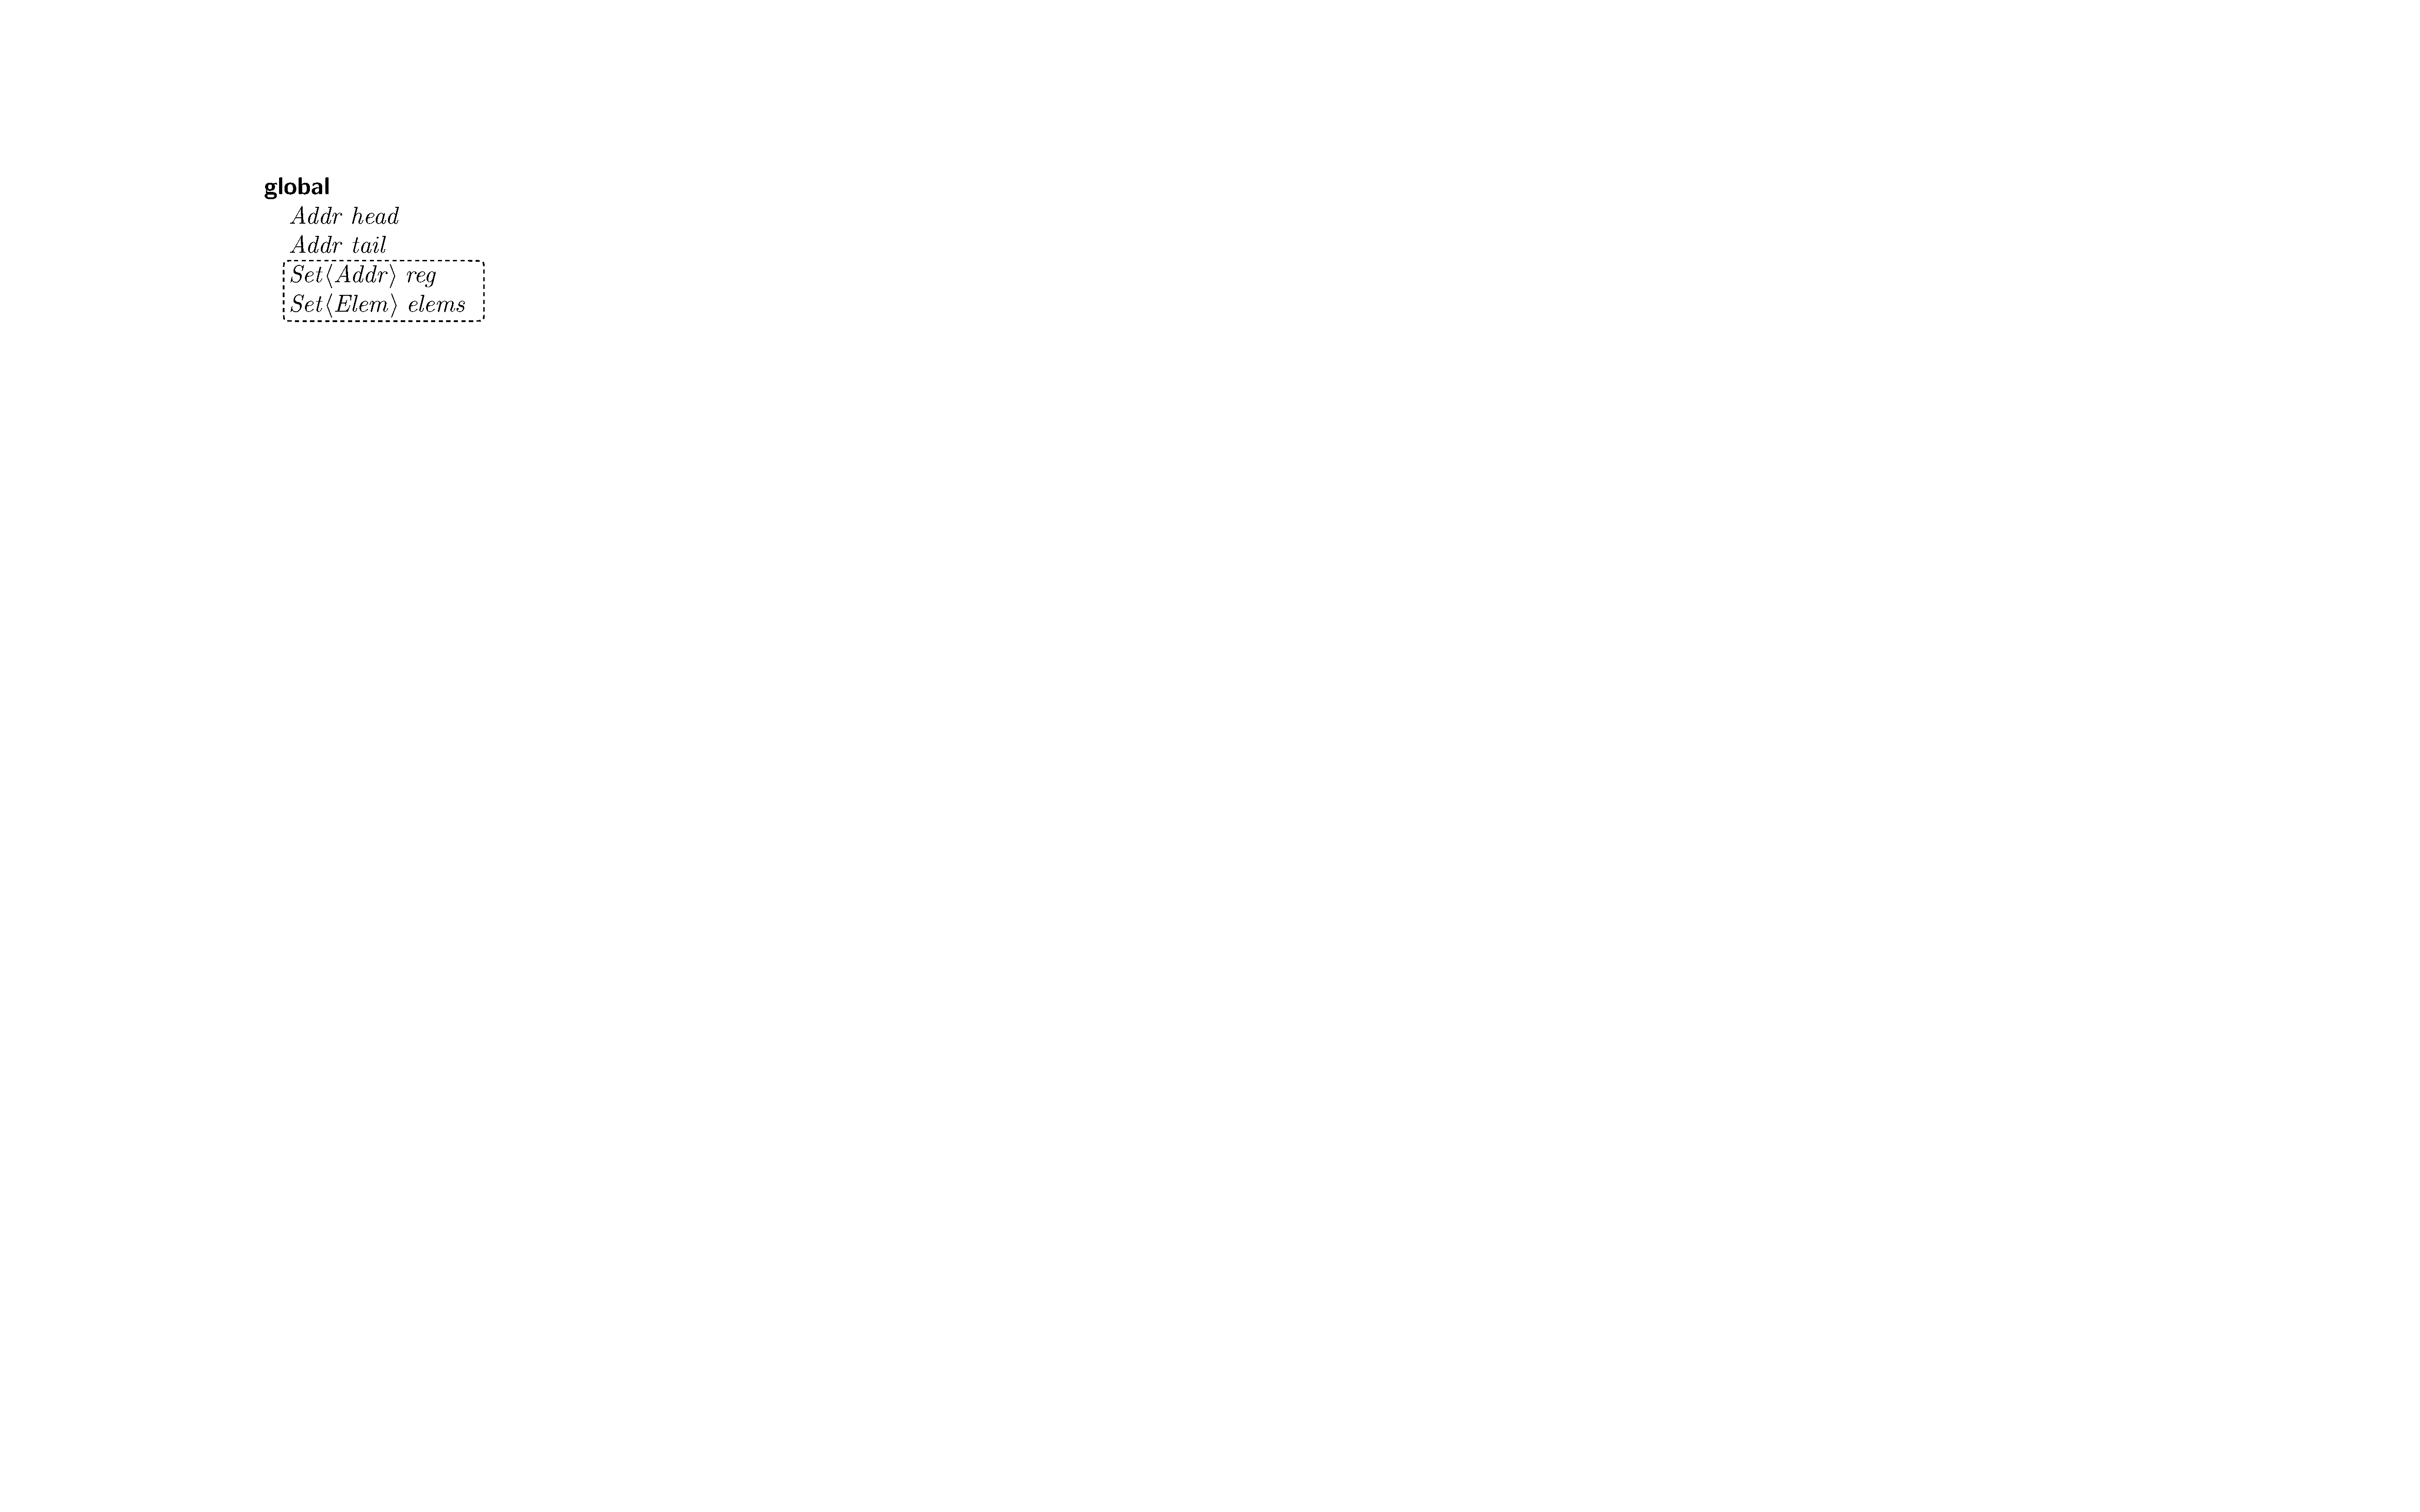
\includegraphics[scale=\figscale]{graphics/_lists_classes}
\end{center}
%
The declared global program variables are:
%
\begin{enumerate}
		\item A variable \head, of type address, which points to the 
			first node of the list which has the lowest possible value ($-\infty$).
		\item A variable \tail, of type address, which points to the 
			last node of the list  which has the lowest possible value ($+\infty$).
		\item A ghost variable \region, of type set of addresses, which is 
			used to keep track of the portion of the heap whose cells form the 
			list.
		\item A ghost variable \elements, of type set of elements, which 
			represents the collection of elements stored in the list.
\end{enumerate}


We consider \head and \tail sentinel nodes which are neither removed nor 
modified and we assume that the list is initialized with \head and \tail 
already set.
%
The set \region is initialized containing solely the addresses of \head 
and \tail.
%
Similarly, the set \elements is initialized containing only the elements 
initially stored at the nodes pointed by \head and \tail.
%
There is also a function \concept{havocListElem}() which returns a random element. 

In figure \ref{fig:listcode} we present the program we are going to use, written in \gls{SPL}, with the assume. We can see there are three procedures, \Search, \Insert and \Remove. 

\begin{figure}[!htbp]
		\myframe{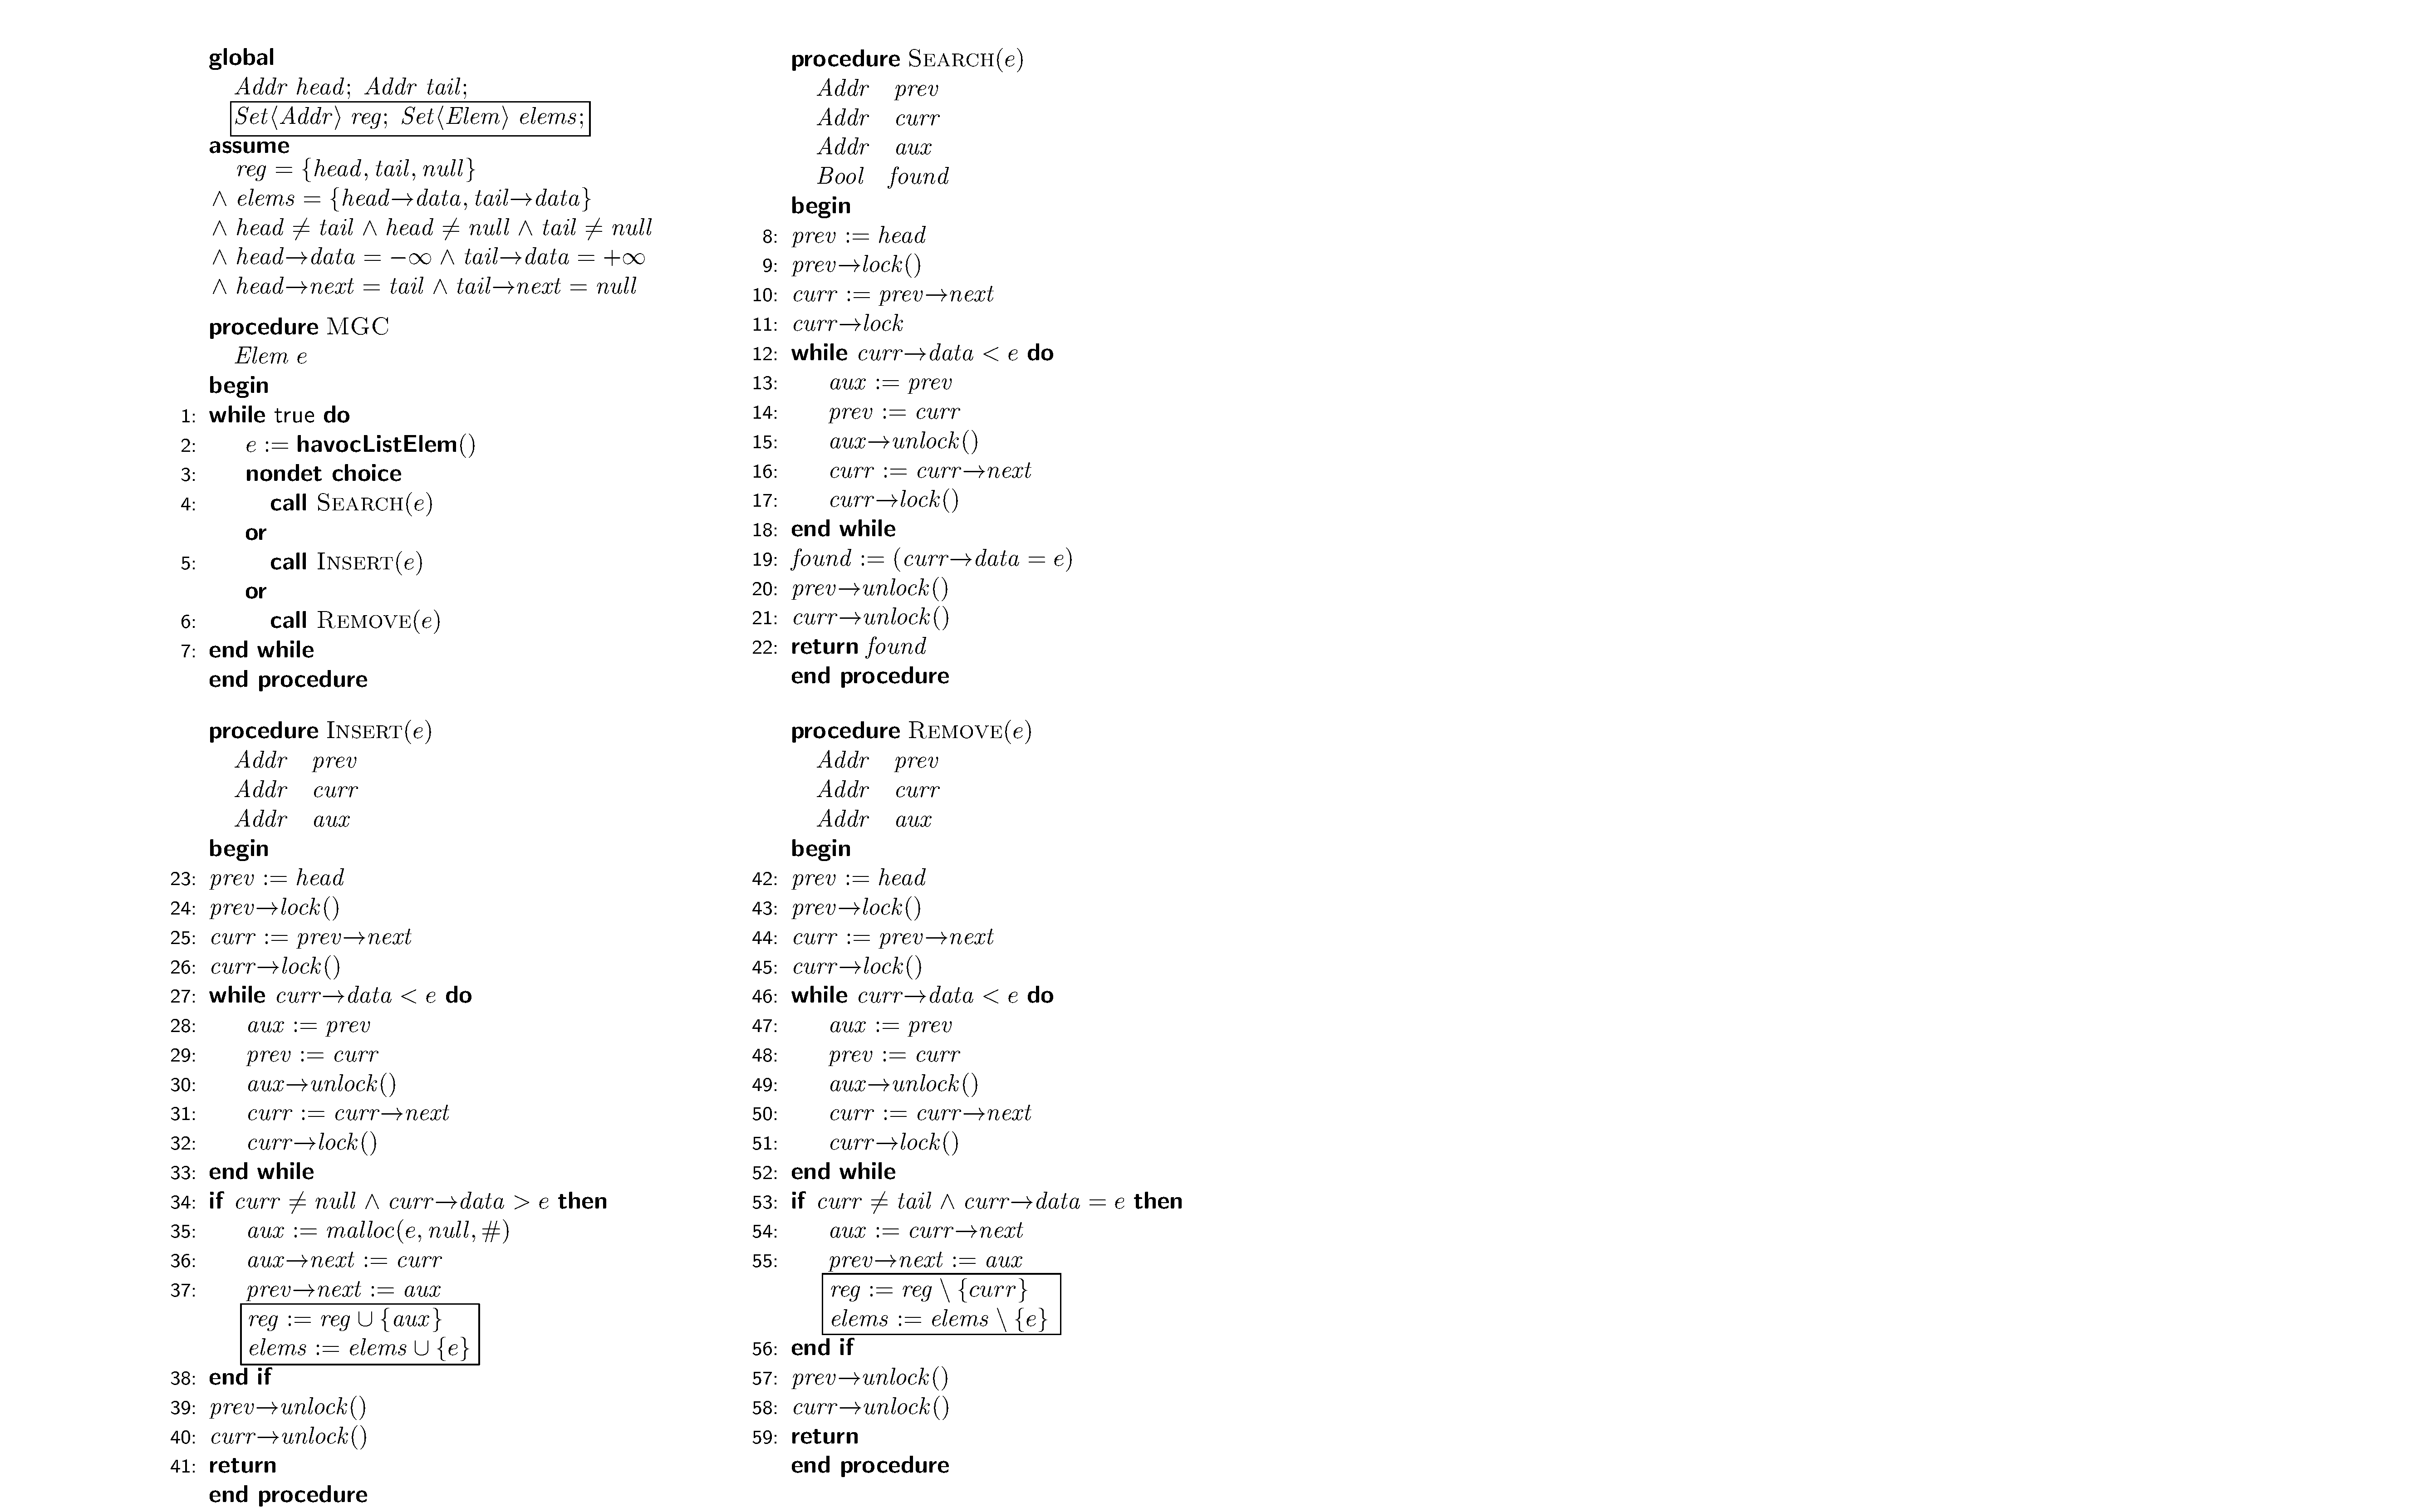
\includegraphics[scale=0.4]{graphics/_listcode}}
		\caption{ Concurrent lock-coupling lists implementation.}
		\label{fig:listcode}
\end{figure}

\subsection{TL3}

\emph{Theory of Linked Lists with Locks} \TLLpL, is the theory we use for describing linked-list heap memory layout. \TLLpL is a multi-sorted first-order theory.

Its definition can be found in \citeapos{paperAle} and \citep[6.2]{thesisAle}


\subsection{Invariants}


